\chapter{Marco Teórico}\label{chapter01}

El crecimiento del comercio electrónico durante los últimos años produjo una transformación significativa en la manera en que consumidores, vendedores y empresas interactúan dentro de plataformas digitales. Los marketplaces modernos concentran millones de productos, búsquedas y transacciones diarias, generando grandes volúmenes de información capaces de reflejar tendencias de consumo, variaciones de demanda y cambios en el comportamiento del mercado.

En este contexto, la información generada por la actividad de los usuarios dentro de entornos digitales no solo permite describir comportamientos ya ocurridos, sino que también puede funcionar como una señal temprana para anticipar cambios de demanda. En trabajos como el de \textcite{KulkarniKannanMoe2012}, los datos de búsqueda en línea son utilizados para anticipar ventas de productos nuevos, lo que refuerza la utilidad de observar señales digitales antes de que una tendencia se encuentre completamente consolidada.

Dentro de este contexto, Mercado Libre representa uno de los ecosistemas comerciales más importantes de América Latina. Su infraestructura reúne vendedores, compradores y productos pertenecientes a múltiples categorías, convirtiéndose en una fuente extremadamente valiosa de información relacionada con consumo digital y comportamiento comercial.

A pesar del gran volumen de información disponible, uno de los principales problemas detectados es la dificultad para identificar productos emergentes de manera temprana. La mayoría de las herramientas actuales únicamente muestran tendencias instantáneas o rankings superficiales, sin construir datasets históricos persistentes capaces de alimentar modelos predictivos o sistemas avanzados de inteligencia comercial.

Como consecuencia, muchos vendedores y emprendedores ingresan tarde a tendencias ya consolidadas, perdiendo oportunidades comerciales debido al aumento de competencia y reducción de márgenes de rentabilidad.

Frente a esta problemática, el presente proyecto propone el desarrollo de una plataforma inteligente capaz de detectar tempranamente productos emergentes mediante la utilización exclusiva de la API oficial de Mercado Libre, mecanismos automatizados de minería de datos y análisis temporal basado en datos históricos construido internamente.

La solución propuesta busca transformar señales dispersas provenientes del marketplace como tendencias, búsquedas, publicaciones, precios y categorías en información estructurada y utilizable para la toma de decisiones comerciales.

En el proyecto, el término ``tendencia'' no se utiliza como sinónimo de ranking instantáneo, sino como una variación observable y sostenida en el tiempo. Cuando se menciona ``búsquedas'', se hace referencia a resultados públicos obtenidos desde endpoints oficiales de búsqueda y no a datos privados de comportamiento de usuarios. Por lo tanto, la detección se apoyará en variables accesibles y registrables como frecuencia de aparición, variación de cantidad de publicaciones, permanencia en listados, evolución de precios, categoría asociada y cambios relativos frente a períodos anteriores.

El enfoque planteado se sostiene sobre tres ejes principales: la recolección automatizada de información accesible desde fuentes oficiales, la construcción progresiva de un histórico propio y el análisis temporal de variables que puedan funcionar como indicios de crecimiento. Esta decisión permite diferenciar el proyecto de una herramienta meramente descriptiva, ya que el valor principal no se encuentra solo en mostrar datos actuales, sino en observar su evolución y detectar comportamientos emergentes.

\section{Concepto central}

Desarrollar una plataforma inteligente capaz de detectar tempranamente productos emergentes en Mercado Libre mediante la recolección automatizada de datos provenientes de su API oficial, la construcción de un dataset histórico propio y el análisis temporal utilizando métricas descriptivas y modelos supervisados de aprendizaje automático.

A los fines del proyecto, un producto emergente será aquel que, durante una ventana temporal definida, presente crecimiento sostenido en frecuencia de aparición, permanencia y/o publicaciones asociadas, con variaciones de precio o categoría que permitan diferenciarlo de aumentos aislados. Esta definición convierte la idea general de tendencia en un conjunto de indicadores medibles a partir del histórico propio.

\section{Decisiones técnicas}

Las decisiones técnicas adoptadas dentro del proyecto responden principalmente a la necesidad de garantizar escalabilidad, automatización, persistencia histórica y capacidad analítica.

Para eso, se plantea una arquitectura basada en APIs REST oficiales, permitiendo acceder a información estructurada y confiable proveniente del marketplace. Asimismo, la construcción de datasets históricos resulta fundamental para realizar análisis temporales y detectar patrones de crecimiento sostenido.

Por otro lado, la incorporación de técnicas de minería de datos permite extraer información relevante a partir de grandes volúmenes de datos, mientras que el uso de modelos supervisados posibilita analizar comportamientos emergentes y diferenciar tendencias reales de variaciones temporales aisladas.

Finalmente, la implementación de dashboards analíticos y mecanismos de monitoreo contribuye a mejorar la visualización de métricas, el seguimiento de tendencias y la disponibilidad operativa de los servicios utilizados.

\section{Alcance}

El proyecto se enfoca exclusivamente en Mercado Libre Argentina utilizando únicamente información obtenida mediante endpoints oficiales autorizados. La plataforma contempla procesos de captura automatizada, construcción de históricos temporales, monitoreo de endpoints y visualización analítica.

El alcance no incluye scraping, acceso a datos privados de usuarios ni predicción directa de ventas internas de Mercado Libre. La plataforma trabajará únicamente con datos disponibles mediante API oficial y con el histórico construido por el propio sistema.

\section{Tecnologías utilizadas}

\subsection{APIs REST}

Las APIs REST constituyen uno de los mecanismos de comunicación más utilizados dentro de arquitecturas distribuidas modernas. Su utilización permite el intercambio estructurado de información entre sistemas mediante protocolos estándar como HTTP.

En el contexto del comercio electrónico, las APIs facilitan el acceso automatizado a información relacionada con productos, búsquedas, tendencias y categorías, permitiendo construir soluciones analíticas basadas en datos externos confiables y actualizados.

La API oficial de Mercado Libre representa la principal fuente de información utilizada dentro del proyecto, ya que permite acceder de manera estructurada a distintos recursos del marketplace mediante autenticación y solicitudes controladas.

\subsection{Minería de Datos}

La minería de datos comprende el conjunto de técnicas orientadas a descubrir patrones, relaciones y comportamientos relevantes dentro de grandes volúmenes de información.

En plataformas de comercio electrónico, estas técnicas permiten identificar productos con crecimiento sostenido, detectar cambios en tendencias de consumo y analizar comportamientos asociados a la demanda del mercado.

Su aplicación resulta especialmente importante en escenarios donde existe una gran cantidad de datos dispersos y dinámicos, ya que posibilita transformar información no estructurada en conocimiento útil para la toma de decisiones.

Dentro del proyecto, la minería de datos constituye uno de los pilares principales para la construcción de históricos y el análisis de productos emergentes.

\subsection{Series Temporales}

Las series temporales representan secuencias de datos organizadas cronológicamente. Su análisis permite estudiar la evolución de determinadas variables a lo largo del tiempo e identificar patrones de crecimiento, estacionalidad y cambios de comportamiento.

En el ámbito del comercio electrónico, el análisis temporal resulta fundamental para comprender cómo evolucionan las tendencias de consumo y detectar variaciones sostenidas en productos o categorías específicas.

Variables como frecuencia de aparición, crecimiento progresivo, cambios de ranking o variaciones de precio pueden utilizarse como indicadores de comportamiento emergente, permitiendo construir métricas orientadas a la detección temprana de tendencias.

Los trabajos sobre predicción de demanda y series temporales, como el de \textcite{LimArikLoeffPfister2021}, muestran la importancia de considerar la evolución histórica de múltiples variables para analizar escenarios de comportamiento futuro.

\subsection{Machine Learning Supervisado}

El aprendizaje automático supervisado permite desarrollar modelos capaces de identificar patrones y realizar clasificaciones a partir de datos previamente etiquetados.

En proyectos orientados al análisis de tendencias, estos modelos pueden utilizarse para reconocer comportamientos asociados a productos emergentes, diferenciar tendencias reales de fluctuaciones temporales y generar estimaciones probabilísticas basadas en datos históricos.

La utilización de variables temporales y métricas descriptivas permite construir modelos con capacidad de aprendizaje progresivo, aportando mayor precisión en la identificación de oportunidades comerciales.

En una primera etapa, el proyecto prioriza métricas descriptivas y reglas de análisis temporal. Posteriormente, esas variables podrán utilizarse como entrada de modelos supervisados, por ejemplo para clasificar productos según su probabilidad de presentar crecimiento sostenido. Esta decisión es consistente con trabajos como el de \textcite{ElalemMaierSeifert2023}, donde se analiza la predicción de productos nuevos con ciclos de vida cortos y disponibilidad limitada de datos históricos.

\section{Stack tecnológico preliminar}

El stack tecnológico se define de manera preliminar para bajar la arquitectura a decisiones más concretas, sin cerrar completamente futuras modificaciones de implementación.

\begin{table}[ht]
	\centering
	\caption{Stack tecnológico preliminar}
	\label{tab:stack}
	\begin{tabularx}{\textwidth}{@{}>{\raggedright\arraybackslash}p{2.6cm} >{\raggedright\arraybackslash}p{4.2cm} X@{}}
		\toprule
		\textbf{Componente} & \textbf{Tecnología propuesta} & \textbf{Justificación} \\
		\midrule
		Frontend & Next.js (React + TypeScript) & Permite construir dashboards web con componentes reutilizables y tipado estático. \\
		Backend & Next.js (API Routes) + TypeScript & Facilita exponer servicios REST y conectar la lógica de negocio con el análisis de datos. \\
		Captura de datos & Node.js + consultas a API oficial & Permite automatizar solicitudes controladas a Mercado Libre sin depender de scraping externo. \\
		Persistencia & PostgreSQL (Supabase) + Prisma ORM & Permite almacenar información estructurada e históricos temporales con consultas relacionales. \\
		Análisis & Python (Pandas + Scikit-Learn) para la etapa de ML & Herramientas ampliamente utilizadas para procesamiento de datos y modelos supervisados. \\
		Visualización & Dashboard web & Permite presentar tendencias, métricas y alertas en una interfaz comprensible para el usuario. \\
		\bottomrule
	\end{tabularx}
\end{table}

\section{Evolución de las decisiones técnicas}

Durante la implementación del prototipo, el stack preliminar fue ajustado: el backend y la captura de datos se desarrollaron finalmente sobre Next.js (API Routes) y Node.js, unificando frontend y backend en un único lenguaje (TypeScript) y un único despliegue, lo que reduce la complejidad operativa del proyecto. La capa de persistencia (PostgreSQL, gestionada mediante el ORM Prisma) y la arquitectura general de componentes (captura \(\rightarrow\) base histórica \(\rightarrow\) motor analítico \(\rightarrow\) API \(\rightarrow\) dashboard) se mantienen sin cambios: se modificó la herramienta de implementación, no el diseño. Python (Pandas + Scikit-Learn) queda reservado para el motor analítico y de Machine Learning de la etapa siguiente, que se integrará leyendo directamente la base histórica PostgreSQL.

\section{Arquitectura General}

La arquitectura del sistema se encuentra organizada en distintos componentes que trabajan de manera integrada para permitir la captura, procesamiento, almacenamiento y visualización de información relacionada con tendencias comerciales.

El frontend cumple la función de representar la información de manera visual e intuitiva, permitiendo interpretar tendencias, métricas temporales y variaciones de comportamiento de los productos. La visualización de datos resulta fundamental para facilitar la toma de decisiones y transformar grandes volúmenes de información en indicadores comprensibles para el usuario (ver Figura~\ref{fig:diagrama-componentes}, \emph{Dashboard (React)} dentro del Carril 2).

Por otro lado, el backend actúa como el componente encargado de administrar el procesamiento general de la plataforma. Su función principal consiste en organizar la información obtenida, coordinar los distintos procesos internos y garantizar el correcto funcionamiento de la lógica del sistema (ver Figura~\ref{fig:diagrama-componentes}, \emph{API REST (API Routes)} dentro del Carril 2).

El motor de minería de datos representa uno de los elementos centrales del proyecto, ya que permite automatizar la obtención y análisis de información proveniente del marketplace. Su importancia radica en la capacidad de detectar patrones, registrar cambios temporales y construir históricos que luego pueden utilizarse para identificar comportamientos emergentes (ver Figura~\ref{fig:diagrama-componentes}, subsistema \emph{Captura automatizada -- Carril 1}).

La persistencia de datos cumple un rol clave dentro de la plataforma debido a que posibilita almacenar información histórica de manera organizada y continua. Mantener registros temporales permite realizar comparaciones, analizar evolución de tendencias y generar bases de información útiles para futuros modelos analíticos (ver Figura~\ref{fig:diagrama-componentes}, componente \emph{Base Histórica}; el detalle de las tablas se muestra en la Figura~\ref{fig:diagrama-er}).

Finalmente, el monitoreo contribuye a garantizar estabilidad y disponibilidad dentro del sistema, permitiendo controlar el comportamiento de los servicios utilizados y detectar posibles interrupciones o variaciones que puedan afectar la recolección de información (ver Figura~\ref{fig:diagrama-componentes}, \emph{probe\_endpoints.js} dentro del Carril 1).

La arquitectura opera además en dos carriles complementarios. El primero es el carril de captura en segundo plano: los procesos programados que construyen el histórico de manera sistemática y controlada, tres veces por día. El segundo es un carril de consulta en tiempo real: desde el dashboard, el usuario puede buscar productos puntuales consultando la API oficial en vivo, sin esperar a la próxima corrida de captura. Esta separación protege la recolección sistemática (cuyo ritmo está calibrado para respetar los límites de la API) de la carga variable de las consultas interactivas, y permite contrastar el histórico propio con el estado instantáneo del marketplace (ambos carriles se distinguen en la Figura~\ref{fig:diagrama-componentes}).

\subsection{Diagrama de componentes propuesto}

\begin{figure}[ht]
	\centering
	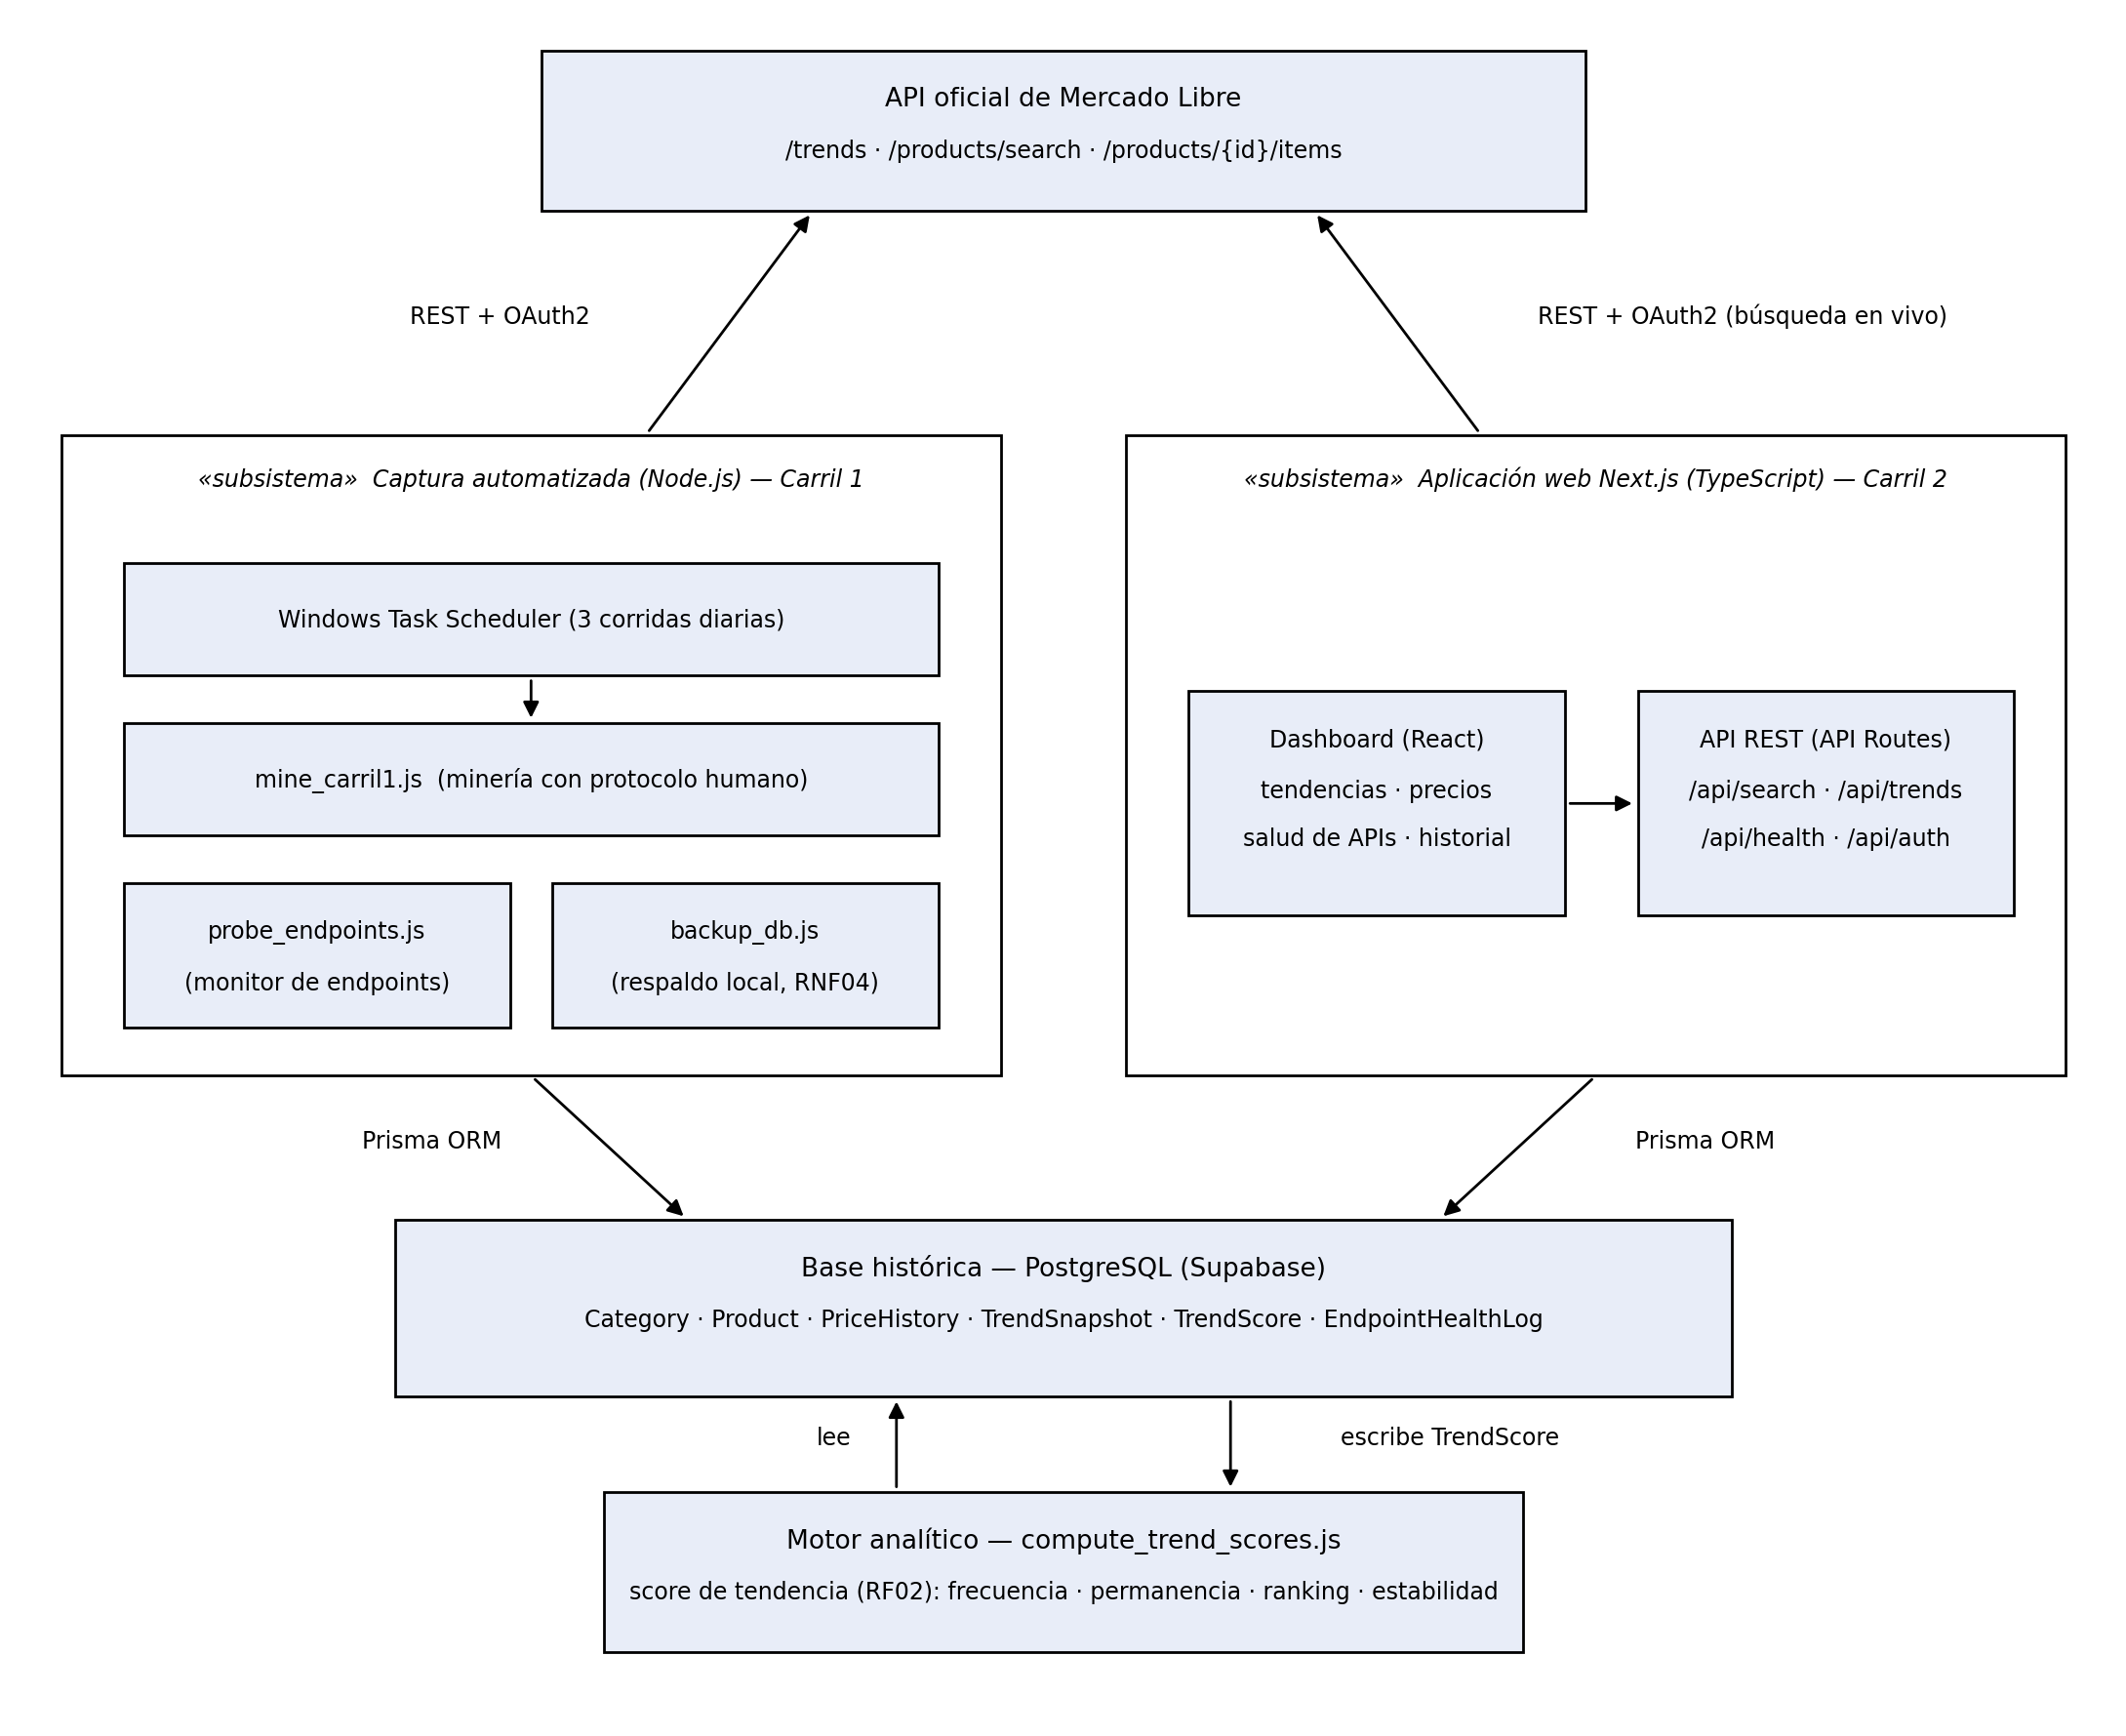
\includegraphics[width=0.95\textwidth]{./images/diagramas/diagrama_componentes.png}
	\caption{Diagrama de componentes del sistema.}
	\label{fig:diagrama-componentes}
\end{figure}

El flujo de datos comienza con consultas periódicas a la API oficial de Mercado Libre. Luego, la información recolectada se almacena en una base histórica. A partir de ese histórico, el motor analítico calcula métricas temporales que permiten identificar productos con crecimiento sostenido o cambios relevantes. Finalmente, el backend expone esos resultados para que el dashboard los presente de manera visual (flujo completo en la Figura~\ref{fig:diagrama-componentes}).

\subsection{Diagrama de Clases (UML)}

El diagrama de clases representa las principales entidades del sistema y sus relaciones (ver Figura~\ref{fig:diagrama-uml}).

\begin{figure}[ht]
	\centering
	
\includegraphics[width=0.85\textwidth]{./images/diagramas/diagrama_clases_uml.png}
	\caption{Diagrama de clases UML del sistema.}
	\label{fig:diagrama-uml}
\end{figure}

\subsection{Modelo de Datos -- Diagrama Entidad-Relación}

El modelo de datos se implementa sobre PostgreSQL. El diagrama Entidad-Relación muestra las tablas principales y sus relaciones (1:N) (ver Figura~\ref{fig:diagrama-er}).

\begin{figure}[ht]
	\centering
	
\includegraphics[width=0.9\textwidth]{./images/diagramas/diagrama_er.png}
	\caption{Diagrama Entidad-Relación del modelo de datos.}
	\label{fig:diagrama-er}
\end{figure}

\section{Modelos y Arquitecturas Aplicables}

El desarrollo de plataformas inteligentes orientadas al análisis de tendencias requiere la utilización de arquitecturas capaces de procesar información de manera distribuida, escalable y organizada. En este contexto, los modelos basados en arquitecturas cliente-servidor y servicios desacoplados permiten separar responsabilidades entre captura de datos, procesamiento, persistencia y visualización de información.

La arquitectura cliente-servidor constituye uno de los modelos más utilizados dentro de aplicaciones modernas debido a su capacidad para dividir el sistema en componentes especializados. El frontend se encarga de la interacción con el usuario y visualización de resultados, mientras que el backend administra la lógica de negocio, procesamiento de información y comunicación con servicios externos.

Dentro del proyecto, este enfoque permite organizar la plataforma en módulos independientes capaces de trabajar de manera coordinada. La captura automatizada de información proveniente de Mercado Libre se realiza mediante procesos específicos de minería de datos, mientras que el backend administra el almacenamiento histórico, la generación de métricas y el monitoreo de disponibilidad de endpoints.

Además, el uso de APIs REST como mecanismo de integración favorece la interoperabilidad entre sistemas y simplifica el intercambio de información estructurada mediante solicitudes HTTP y respuestas en formato JSON. Este modelo de comunicación se consolidó como estándar en aplicaciones distribuidas debido a su flexibilidad, escalabilidad y facilidad de integración con múltiples tecnologías.

Por otra parte, la utilización de arquitecturas basadas en procesamiento de datos temporales resulta especialmente relevante en sistemas de análisis predictivo. La construcción progresiva de datasets históricos permite transformar eventos aislados en información acumulativa capaz de reflejar patrones de crecimiento, cambios de comportamiento y tendencias emergentes.

En proyectos orientados a inteligencia comercial, estas arquitecturas permiten incorporar posteriormente modelos de aprendizaje automático, motores analíticos y dashboards interactivos sin necesidad de rediseñar completamente la estructura principal del sistema. De esta manera, la arquitectura no solo cumple una función técnica, sino que también condiciona la capacidad futura de expansión y evolución de la plataforma.

\section{Métricas y Análisis Temporal}

El análisis temporal constituye uno de los componentes centrales en sistemas orientados a la detección de tendencias y comportamiento emergente. A diferencia de los análisis estáticos, las métricas temporales permiten observar cómo evolucionan determinados fenómenos a lo largo del tiempo, facilitando la identificación de patrones de crecimiento, estacionalidad y cambios abruptos en la demanda.

Dentro del comercio electrónico, las variaciones temporales representan señales fundamentales para comprender el comportamiento del mercado. Factores como el aumento sostenido de publicaciones, la frecuencia de aparición de determinados productos, las variaciones de precio y los cambios de ranking pueden reflejar el inicio de nuevas tendencias comerciales antes de que se consoliden masivamente.

En este proyecto, el análisis temporal se basa principalmente en la construcción de datos históricos propios obtenidos mediante la API oficial de Mercado Libre. La persistencia de información cronológica permite comparar comportamientos entre distintos períodos y detectar productos con crecimiento sostenido respecto de su categoría.

Las métricas descriptivas constituyen la primera aproximación para interpretar estos datos. Indicadores como frecuencia de aparición, crecimiento porcentual, permanencia dentro de tendencias y evolución de precios permiten generar una representación cuantitativa del comportamiento de cada producto dentro del marketplace.

A su vez, estas métricas funcionan como base para futuros modelos supervisados de Machine Learning, ya que las variables históricas permiten entrenar algoritmos capaces de diferenciar tendencias reales de aumentos temporales de popularidad. De esta manera, el análisis temporal no solo aporta información descriptiva, sino también capacidades predictivas orientadas a mejorar la toma de decisiones comerciales.

Finalmente, el uso de métricas históricas contribuye a reducir la dependencia de rankings instantáneos o tendencias superficiales, permitiendo construir una visión más consistente y contextualizada del comportamiento del mercado digital.

La detección temprana no se define por la aparición aislada de un producto en un ranking, sino por la repetición de señales durante un período determinado. Por ese motivo, el proyecto prioriza métricas que permitan observar continuidad, intensidad y variación temporal.

\subsection{Métricas preliminares}

\begin{table}[ht]
	\centering
	\caption{Métricas preliminares}
	\label{tab:metricas}
	\begin{tabularx}{\textwidth}{@{}>{\raggedright\arraybackslash}p{3cm} >{\raggedright\arraybackslash}p{4cm} p{1.8cm} X@{}}
		\toprule
		\textbf{Métrica} & \textbf{Descripción} & \textbf{Tipo} & \textbf{Utilidad para el proyecto} \\
		\midrule
		Frecuencia de aparición & Cantidad de veces que un producto aparece en consultas o registros temporales. & Descriptiva & Permite observar presencia sostenida. \\
		Crecimiento porcentual & Variación entre períodos consecutivos. & Descriptiva & Permite identificar aumentos relevantes. \\
		Permanencia en tendencias & Cantidad de períodos en los que el producto mantiene visibilidad. & Descriptiva & Ayuda a diferenciar señales aisladas de tendencias sostenidas. \\
		Evolución de precios & Cambios de precio registrados a lo largo del tiempo. & Descriptiva & Permite analizar comportamiento comercial y competencia. \\
		Variación de publicaciones & Cambios en la cantidad de publicaciones asociadas a un producto o categoría. & Predictiva & Puede indicar aumento de oferta o interés comercial. \\
		Indicador compuesto & Combinación ponderada de métricas anteriores. & Propuesta & Podría utilizarse como base para clasificar productos emergentes. \\
		\bottomrule
	\end{tabularx}
\end{table}
